% Created 2013-05-16 Thu 14:55
\documentclass[11pt]{article}
          \usepackage[margin=0.5in]{geometry}
          \usepackage{graphicx}
          \usepackage{placeins}
          \usepackage{float}
          \usepackage{subfigure}


\title{Report: Where do we go from here?}
\author{Ivar Thorson}
\date{16 May 2013}

\begin{document}

\maketitle


  One of my engineering habits is to periodically review the conceptions of a project in light of what has been learned while working on the project. The purpose of this informal document is to externalize my (mis)conceptions of our goals, and hopefully expose some weak reasoning. 

\section{Rethinking Experimental Goals}
\label{sec-1}


\subsection{The Holy Grail: Predictive Models}
\label{sec-1.1}


   Why are we putting all this work trying to get good predictive model fits? Information theory tells us that if we can predict a neurons behavior precisely, we have learned something important or relevant about that neuron. Yet I'm a little unclear on when we stop the hunt for ever better predictions. Assuming we can predict a neuron's behavior with 95\% accuracy -- where do we go from there? 99.9\%? At what point do we stop looking for the holy grail? Is this information useful to other researchers? Is the end goal to compare NARF-measured behaviorally-induced changes in neural function with mechanistic explanations of neural activity? For example, if we can model the inhibition associated with attentive listening tasks with sufficient precision, and we ask a neural physiologist for data describing the effect of various neurotransmittters, is our goal to say that attentive listening tasks correlate well with models describing altered choline transportation? More to the point, what kind of predictive power would we need to reach that level? What's the minimum we need to do to do real, useful science?

   Or are we trying to get good fits to somehow map out the function of the cortex in more detail? A first step towards understanding is often quantification; even a weak quantification of neural function might help us. What sort of model would let us discover new things in A1, or other regions of the brain? How would we ever map out a region of the brain that is not sensory in nature?

\subsection{Sparse STRFs}
\label{sec-1.2}


   STRFs are both descriptive and predictive -- and they are much easier to interpret when they are sparse. I know we \emph{expect} STRFs to be sparse and with a single dominant peak, but why must this necessarily be so? While a neural representation of sound immediately at the cochlea may be very precise, it is plausible that neurons further up the neural pathway are not spectrally regimented quite so rigidly. Is it possible that we believe that most neurons in A1 are responding to single tones simply because we cannot measure their sensitivity as strongly?

\subsection{Categorization}
\label{sec-1.3}


   At some point before publication, we'll need to come to a conclusion about into which category a neuron falls; neuron A is ``depressing'' neuron, neuron B is a ``linear'' neuron, and neuron C is something else. But do we try all the models and pick them post-hoc? Doesn't that bias us towards finding a model that works just by chance? How exactly will this categorization be determined?

   Much of the interesting science will come in when we can quantify how model parameters change when the animal is in different behavioral states. We have hardly explored this at all, although the capability to study these in depth has been built in to NARF with the multiple parameter set functionality. 

\section{Rethinking Model Structure}
\label{sec-2}


  NARF has seen some major growth in the last 5 months. Now that we are simulating many models a day, it seems like an appropriate time to slow down and question our model assumptions before proceeding further down the current path -- a more promising one may be awaiting us nearby. 

\subsection{Stimulus}
\label{sec-2.1}


   We've been so focused on modeling that we have lost sight of our ability to choose the stimulus and feature set we give to those models. What modifications could we make to the inputs to our models?

\subsubsection{Stimulus Envelope}
\label{sec-2.1.1}

    
    The stimulus envelope has proven to be a reliable feature from which to predict neural activity since it shows the intensity of a single frequency band. But we haven't criticized it in a while so recall to mind its limitations. First, in the particular implementation we are using, the stimulus envelope is not being extracted from the WAV file presented to the ferret, but is rather taken directly from the modulation used to generate the WAV file. Although the correlation between the two is probably very high, since this is random noise we are modulating, there is a possibility that the stimulus envelope used to generate the WAV and the actual stimulus envelope present in the WAV are different in some respect. Also, perhaps neurons are \emph{not} perfect at reconstructing a sound envelope and have some biases that make them unable to catch modulations faster or slower than some limit. Predictions based on this neurally undetectable information may be decreasing our predictive performance.

\subsubsection{Stimulus Prestim Silence}
\label{sec-2.1.2}


    The stationary dynamics of the (time invariant) neural models we are using poorly track the first second or so of the stimulus because neurons undergo a huge shift in their internal state during that period. It is obvious that a rested neuron and a neuron that just fired repeatedly will respond to an identical stimulus differently. However, when we tested the effect of removing prestim silence on batch 240, only 9 of 38 neurons showed any improvement. Every single one of those 9 neurons had ``low saturation'' nonlinearities. Is this a coincidence? Do we see changes in the nonlinearities if we omit the first second of data?
    
    I've said before that it's probably my imagination, but my gut says that many neurons seem to exhibit very strange behavior in stimulus \#1, the very first edge (right after the sound begins). These are never tracked as close as the onsets of other stimuli, and I think it's because there is more than 0.5s of prestim silence. Chronological order very likely \emph{matters} to neurons, and I don't really like the idea of randomizing them for no good reason. Are they being randomized? 

\subsubsection{Multiple Frequency Channel Interaction}
\label{sec-2.1.3}


    Batches 240 and 242 are stimulating neurons in a very limited way: using bandpass filtered noise chosen to match the peak sensitivity of a neuron. Most of the neurons show only a single peak in the STRF. As I asked earlier: is this an artifact of the way STRFs are computed, or is it a fundamental truth about the way neurons in A1 behave? I can imagine that these artificial stimuli we are presenting are not driving some cells very well. It seems conceivable that some neurons respond well only to two-frequency stimuli, for example. If A is one frequency and B is another frequency, are there neurons that fire when both (A AND B) are present? Are there neurons that fire when ether or both is present (A OR B)? Are there pathological neurons that fire only when one but not both are present (A XOR B)? The latter case could not be predicted with a linear filter, I believe.

\subsubsection{Pitch-Selective Neurons}
\label{sec-2.1.4}


    While helping Daniela with her homework, I learned about how some neurons are pitch-sensitive and essentially fire in a way that suggests they can reconstruct a missing or attenuated fundamental frequency of a natural sound from its harmonics. I immediately imagined this phenomenon occurring as some sort of second-order effect resulting from combinations of frequency-sensitive neurons. Graphically, it would be something like this:
    
    \begin{center}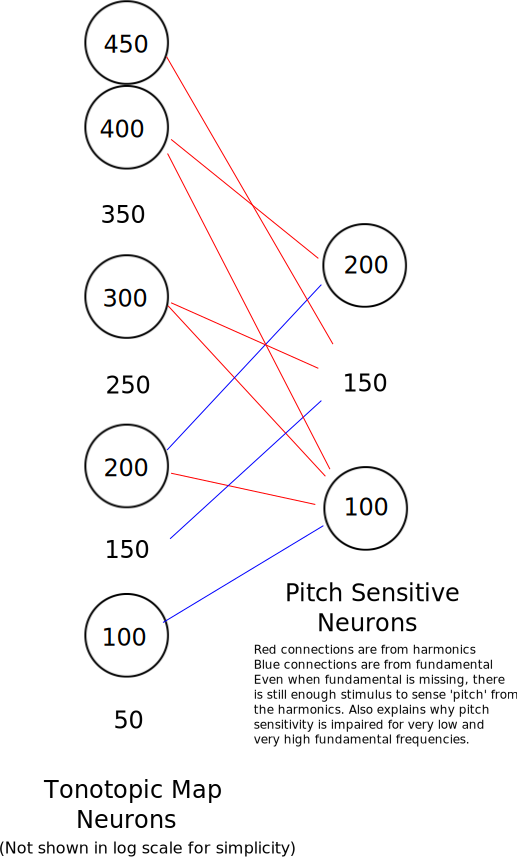
\includegraphics[height=5in]{pitch-sensitive-neurons.pdf}\end{center}

    Admittedly, this is a pretty crude notion and probably a million other people have already done careful experiments that explain pitch sensitivity in more nuance. I'm just wondering that if we had higher-resolution ways of getting STRFs that showed multiple sensitive frequencies, and we presented natural spectrally-rich and harmonically correlated stimuli (both with and without the fundamental frequency) to the ferrets, is it possible that we might find some neurons in A1 that are more pitch-sensitive than frequency-sensitive? Would the latencies of such neurons compared to the latency of purely frequency-sensitive neurons tell us anything about their connectivity?

\subsubsection{Wavelet Feature Extraction}
\label{sec-2.1.5}


    Wavelets can be used to express a huge variety of transformations, expressing bandpass information, describing latency, and performing very general (linear) transformations. It's possible that using NARF to fit wavelets might reveal precise information about the exact auditory features to which a neuron is responding. Such a model could subsume the current function of computing the envelope, the compressor, and the FIR filter. The wavelet would probably have to be parametrized in some way -- even just a 20ms-long filter at 50KHz sampling rate would have 1000 dimensions which would need to be fit.
    
    For example, one biologically plausible parametrized wavelet is the gammatone filter. These are basically just wavelets which express a center frequency, frequency band width, with peak amplitude phase locking or not. Their envelope already expresses some of the functionality of logarithmic compression, since it is based on an exponential.

\subsection{Peri-stimulus Time Histograms (PSTH)}
\label{sec-2.2}


   We have almost exclusively been using a 100Hz-sampled PSTH called RESPAVG as the reference with which to compare our predictions. What alternatives do we have to continuing to use this as our reference?

\subsubsection{Bin Size}
\label{sec-2.2.1}


    One question we have hardly addressed at all is how model fits differ when RESPAVG is binned at smaller intervals than 10ms (100Hz). Trying 5ms (200Hz), 3.33ms (300Hz), or even 2ms (500Hz) could give us more resolution into what is happening even if it makes our prediction scores look less impressive.

\subsubsection{Averaging}
\label{sec-2.2.2}


    Our model predictions are compared to the averaged response signal RESPAVG. Using an average is not a bad idea given sufficient quantities of data, but for sparse signals perhaps there is extra information that could be cleaned from the signal by \emph{not} averaging the trials and taking some performance metric across all the trials independently. For a linear system there it makes no difference if the responses are averaged or not, but for a nonlinear system or especially a system with memory that might not be true. 

\subsubsection{Smoothing}
\label{sec-2.2.3}


    At higher frequencies, I once tried using a Gaussian kernel smoother (actually just a [1 4 1] kernel) to smooth RESPAVG during estimation sets (not validation sets). With 10ms bin sizes, this smeared/smoothed responses slightly to neighboring 10ms bins. The effect on predictive performance was unquestionably negative, and this makes sense since most neural responses are not 10's of milliseconds long. However, at higher frequency rates smoothing may help us avoid over-fitting and be beneficial. It's cheaper than jackknifing, at least!
    
    Of course, a Gaussian is not a very neurologically plausible distribution to smooth with. Using a generalized linear model and a Poisson/exponential curve is another straightforward way to interpolate average firing rates between sampled data. This should probably be done simply at the sampling rate selected, however for maximum extraction of information content from a RESPAVG signal, we could do the smoothing inference with 10KHz resolution. Then, to bring the 10KHz signal back down to the frequency of interest, we could integrate the results in each time bin to determine the final bin value. The only reason this two-step smoothing might be preferred is if a spike occurs close to a bin boundary, under this scheme it would be more fairly distributed between the two bins.

\subsection{Compressors}
\label{sec-2.3}


   Compressors are our pre-FIR nonlinearity, and we chose them rather empirically because they seem to improve our results. Let's revisit some assumptions we made.
   
\subsubsection{Logarithmic and Square Root}
\label{sec-2.3.1}


   The primary motivation for using a compressor nonlinearity is that we believe that neurons respond logarithmically to increasing volume rates. We also know that neurons can't fire faster than some limit, so adding a term to asymptotically approach that maximum rate of fire seems reasonable. but is that really what we are modeling? A simple experiment might help us determine this. For example, if we simply present the same bandpass stimulus at increasing volume levels, can we get a better estimate of the compressor? Maybe it's not described well by the LOG2B keyword at all, and the average rate of fire drops off at the higher volume levels making the curve non-monotonic. We already see many curves like this in the nonparametric nonlinearity curves, and correcting it \emph{before} the FIR filter could show benefits.
   
   Also, I'm not really clear on how an absolute sound intensity (say, 80dB as heard by the ferret) corresponds with the data we are getting from BAPHY. Is BAPHY normalizing the signals before giving them to NARF? Is the absolute sound intensity expressed explicitly in the signal by its magnitude, or are all signal magnitudes scaled to be 1? Is the compressor is always working on data scaled in the same way (i.e. the same volume scale for all neurons)? If not, isn't that a bug? Considering absolute intensity at the compressor stage might improve our fits, even if we normalize before the FIR filter anyway.

   At one point we tried fitting the logarithm and square root along with the other coefficients, but it never seemed to work very well when combined with the FIR coefficients. Perhaps it should be fit in a separate step.

\subsection{Stateful Components}
\label{sec-2.4}


   Currently the only module storing any kind of neural \emph{state} is the depression filter. The fact that it usually improves the fits suggests we should put more work  into finding other simple recursive filters that also have some time-varying state

\subsubsection{Depression Filters}
\label{sec-2.4.1}


    The depression filters are simple, biologically plausible, and exactly the kind of neural modeling that should be done. However, there is a troubling aspect of the depression filter that needs to be considered: the state of the depression filter is probably being estimated in a very poor way. The depression filter state is being estimated ``open-loop'', since it is estimated entirely from input data and there is no correction for actual spiking events that are occurring. From robotics experience, open loop models very poorly track the actual state of a dynamic system, even if their parameters are estimated fairly closely.

    But how can we fairly estimate both the internal state and model parameters at the same time? One of the simplest thing that we could try would be to use a single-pass Kalman filter with a very low weight for the (assumed noisy) neural observations. This would \emph{mostly} estimate the system state based purely on the STIM signal, but would still gently correct for model inaccuracies that would otherwise bring the state greatly out of sync with the actual RESPAVG signal.

    A much slower but more flexible algorithm would be to use Expectation Maximization to estimate the state of the system in the context of a model. Perhaps this should only be done after the fitting is completely done, as it proved too slow for use during fitting.

\subsubsection{Formulation from Linear Feedback Control Theory}
\label{sec-2.4.2}


    There is a huge amount of engineering control theory literature available for studying incrementally linear systems governed by ordinary differential equations of the form:
    
    \[ \dot{x} = Ax + Bu \]
    \[ y = Cx + Du \]

    The equations can be either discrete or continuous. Uppercase letters are matrices, lowercase letters are vectors. In block diagram form, the above model looks like this:

    \begin{center}\includegraphics[width=4in]{Typical_State_Space_model.png}\end{center}

    These types of formulations are well researched and immediately applicable to physical systems of all kinds, including neural models. For simple systems ABCD have constant elements, but in general models the elements of ABCD can be functions of other variables. If $u$ is the history of the last 10 STIM values, then matrix $B$ is effectively our linear filter, assuming it has constant elements. For models with depression terms, we could argue that depression's statefulness and is creating functionality somewhat like the $A$ matrix, assuming that depression was modeled using first-order exponentials. Finally, the nonparametric nonlinearity is somewhat similar to the effect of matrix $C$. Most systems don't have any feed-through terms $D$. Neural systems would never have this block unless we were stimulating neurons electrically and trying to avoid the confounding effect of applied voltage stimulus on the measurement of spikes. 

    There may be some benefit to thinking about neural activity in terms of these matrices ABC(D). Perhaps there is a even linear model for $C$ that would replace the effect of the NPNL by basing it on some hidden state $x$. Such a model would be simpler than the NPNL we have now. 

    More generally, elements of matrices $A,B,C$ can be made arbitrary functions of $x,u$ and very complex versions of this could be studied. Usually formulating mathematical problems in such a form lets you compute gradients, create state observers, and numerically integrate more efficiently.

\subsection{Linear Filters}
\label{sec-2.5}


   These are the real workhorse of the models, but sometimes I wonder how much I am really learning about a neuron from its FIR filter. What are our alternatives?

\subsubsection{Finite Impulse Response (FIR) Filters}
\label{sec-2.5.1}


     The most obvious piece of information we are getting from the FIR filters is the latency, but if there are inhibition/excitation pairs, we can also glean:

\begin{enumerate}
\item Strong excitation by itself means the neuron's activation represents a ``sustained feature''.
\item Strong excitation followed by strong inhibition means the neuron's activation represents a ``sound onset feature''.
\item Strong inhibition followed by excitation means the neuron's activation represents a ``sound conclusion feature''
\end{enumerate}
    Perhaps we can constrain or parametrize the FIR filter bit more to reduce its dimensionality. For constraints, perhaps just limiting the number of coefficients would help. Have we ever seen any important FIR coefficients beyond 70ms latency, for example? Usually anything beyond 50ms looks like depression effects aliasing onto the FIR filter. 

    For parametrization, perhaps using some sum of (inverse/log) Gaussian to describe the STRF would be an efficient encoding. A mean and covariance matrix would describe a sensitive region in an STRF with just a few parameters and could be discretized to arbitrary precision.

\subsubsection{Volterra Filters}
\label{sec-2.5.2}


    Second order filters are beating the simple linear FIR filters, and often the stateful depression filters. We have only been considering channel-to-channel interactions, not temporal interactions. Perhaps considering the second-order interactions of a signal with a slightly delayed version of itself would also improve performance.

\subsubsection{Inhibition/Excitation}
\label{sec-2.5.3}


    We have not explored whether or not separate inhibition/excitation FIR models improve performance. A little work here could pay big dividends. 

\subsection{Nonlinearities}
\label{sec-2.6}

   
   One persistent observation that I have been struck by is the trade-off in complexity between nonlinearity and filter.  Simple filters have complex nonlinearities. complex Nonlinearities make simpler filters.  This suggests that for sparse, clean filters, we should have better NPNLs. So far, enforcing sparsity on the FIR filter and smoothness on the nonlinearity is giving the qualitatively best results. 

   Aside from that, the most important characteristic of the nonlinearity seems to be how well it extrapolates beyond the bounds of the estimation set data. More research into extrapolation could probably improve performance beyond what we have even now. For now, I think just categorizing what has already been tried is sufficient. 

\subsubsection{NPNL}
\label{sec-2.6.1}


    Good performance, fast to compute and very good in general. Its limitation is found at the extremes of the nonlinearity, which are systematically over-estimated on the low side and under-estimated on the high side. Perhaps 

\subsubsection{NPNL2}
\label{sec-2.6.2}


    A two-dimensional version of NPNL for studying interaction between two channels. I don't know much about this yet. It is suffering from data sparsity, or does it have the same problem as NPNL towards the extreme edges of the nonlinearity?

\subsubsection{NPFNL}
\label{sec-2.6.3}


    A Gaussian window filter with a width equal to 1/5th of the nonlinearity's input domain span that is convolved with the correlation between STIM and RESPAVG. It works pretty fast, is not sensitive to outliers during the prestim silence phase, and extrapolates towards the average of the most extreme points, which is usually reasonable. I don't think this can be improved any further given how simple it is. 

\subsubsection{SENL}
\label{sec-2.6.4}


    A Sparse Gaussian mixture model which uses a small number of 1d Gaussian (0.2 relative width) centered at `representative' data points. Unfortunately, since it uses 1D caution's, it generalizes toward zero as you move away from the known data points -- in other words, it will always extrapolate towards zero. Despite this, it did pretty well and is fast enough to be of some practical use. 

\subsubsection{Gaussian Mixtures}
\label{sec-2.6.5}


    The nonlinearity which produces the simplest, prettiest curves that fit the data. Gaussian mixture models uses three or four expectation-maximized 2D Gaussians to create a nonparametric nonlinearity. The general reference implementation I downloaded from a friend (Sylvain) is very slow, but perhaps could be improved through optimization. I would use this for everything if it weren't computationally so demanding because it's just great. Perhaps it could be used only in the final stages of a fit or with quick, single-pass fitters like boosting. 

\subsubsection{Explicit functions}
\label{sec-2.6.6}

    
    We tried exponentials, sigmoids, second order polynomials, and zero threshold levels. Although simple and attractive as analytical descriptions, they can't hold a candle to nonparametric nonlinearity flexibility. It is also striking how much noisier the FIR fits become when a poorly-fitting explicit output nonlinearity is used. Probably they should be fit separately if a clean FIR is desired, despite the fact that fitting them both together typically produced higher performance. 

\subsection{Performance Metrics}
\label{sec-2.7}


   How do we measure performance, and what other metrics should we consider?

\subsubsection{Correlation}
\label{sec-2.7.1}


    At the end of the day, we have been focused about the correlation coefficient. It's great, it's convenient, it's understandable, but it's not the whole story. It's just a single number being used to describe systems with lots of variance. Probably everyone in this lab is familiar with Anscombe's Quartet, which all have the same mean, variance, regression line, and correlation:

    \begin{center}\includegraphics[width=4in]{anscombes_quartet.png}\end{center}

    Perhaps we need to start at saving other metrics in the NARF browser as well or plotting these correlation diagrams to double-check. Or, automatically detecting and excluding very rare points from the correlation process before computing the final correlation could also give a more accurate metric about the model performance.

\subsubsection{Mean Squared Error (L2 Loss Function)}
\label{sec-2.7.2}


    Like correlation, MSE is sensitive to outliers. Not much else to say about this other than it's a useful metric and that it works pretty well since it controls the absolute scale of model parameters better than simple correlation.

\subsubsection{Absolute Error (L1 Loss Function)}
\label{sec-2.7.3}

    
    Absolute error is something so simple to implement that we should just try it. It's much less sensitive to outliers than the L2 norm and might give qualitatively better FIR fits.

\subsubsection{Maximum Likelihood}
\label{sec-2.7.4}


    My Bayesian education really craves for a \emph{real} performance metric that is probabilistic in some sense. Computing this would give us the Akaike Information Criterion (AIC) and the Bayesian Information Criterion (BIC) metrics as a side effect. Some foundational work to estimate this is already in place (time scaling and inter-spike-interval computation), but I haven't gotten this working with NARF yet. 

\subsubsection{Sparsity Metrics}
\label{sec-2.7.5}


    The FIR sparsity metric currently being used ($d$) is defined as the ratio of the $L_1$ norm to $L_2$ norm, squared. $d$ can vary from a minimum of 1 to a maximum of $n$, where $n$ is the number of parameters. It is thus a comparable metric regardless of how many degrees of freedom $n$ there are -- if the sparsity number $d=3.1$, then it has a dimensionality or complexity of about 3 strong coefficients, and all other coefficients are assumed to be zero. It cannot go below one, the limit at which all the mass of the `mass' of the filter coefficients is concentrated into a single coefficient. 

  The definition is very simple:

  \begin{equation}
  d=\left(\frac{\left\Vert c\right\Vert _{1}}{\left\Vert c\right\Vert _{2}}\right)^{2}
  \end{equation}

  where $\left\Vert c\right\Vert _{1}$ and $\left\Vert c\right\Vert _{2}$ are the one and two norms

  \begin{equation}
  \left\Vert c\right\Vert _{1}=|c_{1}|+|c_{2}|+...+|c_{n}|
  \end{equation}

  \begin{equation}
  \left\Vert c\right\Vert _{2}=\sqrt{c_{1}^{2}+c_{2}^{2}+...+c_{n}^{2}}
  \end{equation}
 
  Finally, if all the coefficients are zero, then $d=n$ because all coefficients are equal. 

  In practice, this metric seems to work appropriately well on the neural data. Probably other people have a proper name for this metric since it is so simple other people must be using it for other purposes as well.
     
\subsection{Fitters}
\label{sec-2.8}


   Most of the time, we have been using single-step fitters. However, the new keyword system should allow us to create models which fit using different algorithms at different times. Also, we should forever keep in mind that ``/There is no globally best fitting routines, only fitting routines which work well for certain cells and models./''

\subsubsection{Annealing (anneal)}
\label{sec-2.8.1}


    Simulated annealing is very slow, but may have some advantages as a fitter when using jackknifes or cross-validation because \textbf{ANNEAL} never finds the same local minimum twice. There is much more variation in jackknifes and would probably allow more shrinkage. 

\subsubsection{Boosting (boost)}
\label{sec-2.8.2}


    Boosting has been our bread and butter for searching through linear coefficients, and gives pretty sparse solutions. The only thing faster than \textbf{BOOST} with early stopping is linear least squares. 

\subsubsection{Line Search (fmin, fminu)}
\label{sec-2.8.3}


    The \textbf{FMIN} keyword and \textbf{FMINU} both use matlab's line search algorithms underneath. The differences seem minor and related to the initialization of the search. Both are pretty robust, although neither converges very quickly. They typically iterate 10000 times and then terminate.

\subsubsection{Linear Least Squares (lsq)}
\label{sec-2.8.4}


    Quick and prone to over-fit, \textbf{LSQ} also tends to give the very best results at high correlations (>0.6) because of its fast convergence. 

\subsubsection{Genetic Algorithm (genetic)}
\label{sec-2.8.5}


    This actually worked pretty well if you add enough generations. There are so many optimization parameters to play with that \textbf{GENETIC} was not fully explored as a fitter. It is probably best left for exceptionally nonlinear problems.
   
\subsubsection{Nonlinear Least Squares (lsqn)}
\label{sec-2.8.6}


    The \textbf{LSQN} keyword uses the nonlinear least squares method underneath. I have not really tested this and am not entirely sure what it is doing, but I guess it is better for moderately nonlinear problems.

\subsubsection{Shrink after Jackknifing}
\label{sec-2.8.7}


    Jackknifing and shrinking are more effective for the lower correlation neurons, as we would expect. Typically only cells with an R value below 0.35 or so see any real benefit from jackknifing. Jackknifing also seems to work better if there is no normalization \emph{after} the FIR filter. It is also more more reliable if there is no nonparametric nonlinearity after the FIR filter. 

    We currently have 4 different implementations which implement jackknifing and shrinking:
\begin{enumerate}
\item \textbf{SHBOO}: Fit 10 jackknifes using boost, then try 100 shrinkage levels on the jackknifes and take the mean of the shrunk jackknifes.
\item \textbf{SHBOO2}: Like shboo, but uses \textbf{LSQ} to fit, and uses 20 jackknifes and 200 final iterations.
\item \textbf{SHBOO3}: Fit 10 jackknifes using boost, take the mean of the jackknifes, then try 100 shrinkage levels on that mean.
\item \textbf{SHBOO4}: Same as shboo3, but using correlation to evaluate performance instead of MSE during the shrinkage
\end{enumerate}
    Shboo3 has equivalent performance to boosting if there is no nonlinearity, and is \emph{slightly} more sparse. If there is a nonlinearity, shboo3 doesn't work as well. This suggests to me that either jackknifing or shrinking (or both) works poorly for non-linearly compensated systems. Perturbing a nonlinear system in two opposite directions and taking the mean of those two points won't necessarily bring you back to where you started, after all. 

\subsubsection{Sparse Bayes Fitter}
\label{sec-2.8.8}

    
    The \textbf{SB} keyword is essentially just gradient descent with a fixed step size, but steps only in the most relevant directions to save time. Since it can never work with sparsity metrics and weighted penalties, I'm inclined to retire it. 

\subsubsection{Sparse Fitters}
\label{sec-2.8.9}


    Computationally extremely slow, it was a brute-force attempt to use a sparseness penalty during the fitting process. By default they use qboost and run 5 jackknifes at 10 different sparsity levels. Out of those 10 sparsity levels, the best jackknifed-averaged parameter set is chosen. They rely on fairly deterministic behavior of the fitters and would do poorly when combined with a random fitter. 
    
\begin{enumerate}
\item sp1boost: take the mean of the jackknifes
\item sp2boost: shrink jackknifes using james-stein
\item sp3boost: shrink jackknifes using stephen's shrinkage equation
\item sp4boost: Use jackknife that best predicts its training set
\item sp5boost: Use jackknife that best predicts the held out data
\end{enumerate}
    
\subsubsection{Automatic Relevancy Detection}
\label{sec-2.8.10}


    I don't know much about it, but if ARD works for nonlinear systems, then this will necessarily be the path to follow. Shrinking just doesn't seem to work well for nonlinear systems.

\subsubsection{Cheating Fitters}
\label{sec-2.8.11}


    For non-Bayesians, it is always cheating to peek at a validation data set. However, it could also argued that we are already cheating because we keep peeking at the validation data set correlation when we select our favorite models, so we are gradually biasing our own results. 

    Perhaps we should explicitly code up our cheating behavior by making an MSES-based fitter which runs at MSES1 through 10 and chooses the sparsity penalty with the highest validation set performance. Generally the MSES\# fits produce the sparsest solutions and at least one of them consistently outperforms plain old MSE. With only 10 peeks at the validation data and given the extreme determinism of boosting and its ability to reliably reach the same minima every time, I doubt we are contaminating our results any more than we already are. However, we should be careful to never use a cheating fitter with a non-deterministic fitter like anneal, because that could end up fitting better just by chance.

    Or we could also grow some Bayesian brains, include our validation data with our estimation data, and start comparing models in terms of ML, or MAP instead of arbitrary metrics like correlation.

\subsection{Initial Conditions}
\label{sec-2.9}


   This is fairly unexplored territory. 

\subsubsection{All Zeros (init0)}
\label{sec-2.9.1}


    In many ways the ideal place to start from when shooting for sparse solutions from scratch, at high sparsity penalty levels it can prevent other coefficients after the first from growing to their proper magnitude. This occasionally locks fitters into absurd local minima at overpoweringly high sparsity levels.

\subsubsection{Reverse Correlation (initrc)}
\label{sec-2.9.2}


    This is a good place to start, although if you use early stopping in the boost algorithm it often leaves a fair amount of ``noise'' in the FIR coefficients as compared to starting from all-zero filter coefficients. 

\subsubsection{All Ones (initones)}
\label{sec-2.9.3}

    
    I mostly used this as a test. It underperforms initrc and init0, not suprisingly. It is probably never useful. 

\subsubsection{Alternated Zeros (init12)}
\label{sec-2.9.4}

    
    I'm not sure as to the purpose of this other than to try to bias the fits of two FIR filters towards one channel or another. Did it work?

\pagebreak
\section{Possible Research Questions}
\label{sec-3}

  
  The following is just a laundry list of questions raised in the previous sections, consolidated in one convenient place. 

\subsection{Stimulus}
\label{sec-3.1}

\begin{enumerate}
\item What is the correlation and MSE between reconstructed envelopes and the envelopes used to generate the WAV? (If I recall correctly, the gammatone filter was correlated to about 0.97 with the envelope.)
\item Could computing a stimulus envelope in another way (via another algorithm) possibly improve performance?
\item Is the stimulus envelope still the only relevant feature to consider, or should we write code that extracts frequency or pitch feature channels?
\item How closely do STRFs derived from a FIR filter of natural stimuli with multiple frequency channels match TORC-derived STRFs?
\item Can much of the envelope, FIR filter, and compressor functionality be subsumed by a single wavelet transformation? How hard is it to fit a wavelet?
\item If we chop off the first second of stimuli, does that qualitatively affect the nonlinearity? What would aliasing effects from non-stationary dynamics look like on a nonparametric nonlinearity?
\item Is it possible that a neuron is sensitive only to paired frequency stimuli in a Boolean way (AND, OR, XOR)?
\item If we performed an experiment presenting spectrally rich sounds possessing pitch -- playing sounds both with and without the fundamental frequency present -- do we find neurons in A1 that have pitch sensitivity?
\end{enumerate}
\subsection{PSTHs}
\label{sec-3.2}

\begin{enumerate}
\item What do fits look like at 100Hz, 200Hz, 300Hz, and 500Hz sampling rates?
\item Does Gaussian Kernel Smoothing improve fits at higher sampling rates?
\item Does Generalized Linear Model Smoothing improve fits at higher sampling rates?
\item Is there any conceivable case where not averaging the responses together would be important? The only one that comes to mind is when computing inter-spike intervals and doing a performance metric based on the shape of the scaled ISI distribution.
\end{enumerate}
\subsection{Compressors}
\label{sec-3.3}

\begin{enumerate}
\item Does removing all normalization of input signals improve compressor fits?
\item Does a sigmoidal compressing nonlinearity do better than SQRT or LOG?
\item Does a non-monotonic compressing nonlinearity have a beneficial effect on prediction?
\item Does an NPNL before the FIR filter have a beneficial effect on prediction?
\item Can compressor parameters be fit separately (perhaps \emph{before} the FIR filter is appended) to improve overall performance?
\item How is absolute sound intensity expressed in the envelope/WAV data we get from baphy? What does the average response vs volume level look like for the entire population of neurons so that we can best choose a single compressor to use by default?
\end{enumerate}
  
\subsection{Stateful Components}
\label{sec-3.4}

\begin{enumerate}
\item Are depression fits different when trained by using non-averaged stimuli presented in their real-life order?
\item How much does fitting the depression filter parameters improve the scores? Can it be done simultaneously with the FIR filter or not?
\item Should stateful components be fitted into an ``excitation depression'' and an ``inhibition depression'' and then recombined?
\item Are ABCD models fittable using standard methods, or will they require some multi-step fitters?
\end{enumerate}
\subsection{Linear Filters}
\label{sec-3.5}

\begin{enumerate}
\item Do the inhibition/excitation models show any clear benefit?
\item Does appending the depression channel create any second-order effects with the linear model?
\item Do considering temporal interactions of a channel with itself improve fits?
\item How sparse are STRF fits of batch 233 (Natural Stimuli)? Do they resemble TORC-generated STRFs?
\item Is parametrizing STRFs from a sum of a limited number of 2D inverse gaussians, poisson curves, etc effective at reducing dimensionality?
\end{enumerate}
\subsection{Output Nonlinearities}
\label{sec-3.6}

\begin{enumerate}
\item Does using an NPFNL with a zeros-flattened left side (anything left of the minimum) improve fits?
\item How sparse is the data given to NPNL2 to estimate the 2D surface?
\item Can NPNL and NPNL2's extrapolation be improved?
\item Can GMM be used in a reasonable amount of time with plain old boosting?
\item How much ``worse'' are explicit functions instead of nonparametric nonlinearities?
\end{enumerate}
\subsection{Performance Metrics}
\label{sec-3.7}

\begin{enumerate}
\item How often are correlation plots not well represented by their outliers?
\item Does a correlation metric that excludes outliers improve our fits?
\item Does an L1 performance metric produce better FIR filters than an L2 norm?
\item Does a weighted average of the L1 norm and the L2 norm produce a better fit?
\item Does the Maximum Likelihood work well as a performance metric?
\item Does the BIC or AIC work well as a performance metric?
\end{enumerate}
\subsection{Fitters and Initial Conditions}
\label{sec-3.8}

\begin{enumerate}
\item Does using correlation instead of MSE during shrinkage improve the end result?
\item Do sp\#boost and shboo\# fitters work better with NONL? (i.e. are they rendered useless by nonlinearities?)
\item If we do a jackknifed fit with the NONL, \emph{then} append the NPNL and shrink, is that more effective?
\item Can GENETIC and ANNEAL be improved by editing the optimization settings?
\item Does a cheating fitter work well with boost? With lsq?
\item Does using multiple fitters in sequence improve correlation scores? (Qboost followed by LSQ, for example)
\end{enumerate}
\pagebreak
\section{Model Possibility Tree}
\label{sec-4}


  In summary, the possibilities I see for models are described by a depth-first search of this tree:
  
\begin{itemize}
\item Stimulus Feature

\begin{itemize}
\item Envelope: \emph{env}

\begin{itemize}
\item Sampling Rate: \emph{100,200,300,400,500}
\item Prestim: \emph{Prestim, noprestim, drop1sec}
\end{itemize}

\item SingleBand: \emph{sell, sgt} (Single band elliptical or gammatone filter)

\begin{itemize}
\item Center: ?
\item Width : \emph{5, 10, 20, 50, 100} (Cents of an octave)
\end{itemize}

\item AllBands: \emph{aell, agt} (All bands elliptical or gammatone filtered)

\begin{itemize}
\item Range: (50Hz - 20KHz, fixed)
\item Bands: \emph{1, 2, 4, 8, 16, 32, 64, 128}
\end{itemize}

\item Pitch: \emph{pitch}

\begin{itemize}
\item Fundamental: ?
\item Harmonics: \emph{3, 5, 7, 9, 11} (Number of harmonics to consider)
\end{itemize}

\item Wavelet: \emph{wavelet}

\begin{itemize}
\item Delay: ?
\item Coefs: 500, 1000, 2000
\end{itemize}

\end{itemize}

\item Response Feature: \emph{sra, srb} (Smoothed respavg, smoothed respavg twopass)

\begin{itemize}
\item Bin size: ? (must match sampling rate)
\item Kernel: \emph{gauss, igauss, exp, gamma}
\end{itemize}

\item Four Part Models

\begin{itemize}
\item Compressors

\begin{itemize}
\item Logs: \emph{log1,2,3,4,5,1b,2b,3b,4b,5b}
\item Sqrts: \emph{root1,root2,root3,root4,root5}
\end{itemize}

\item Depression: \emph{dep, kdep}     (Single depression, with or without kalman correction)

\begin{itemize}
\item DepressionTau: ?
\item RecoveryRate: ?
\item KalmanVariance: ? (amount to trust respavg)
\end{itemize}

\item Linear Filters: \emph{fir, volterra, inex}

\begin{itemize}
\item Coefs: 20ms, 30ms, 50ms, 100ms (history)
\end{itemize}

\item Parameterized Linear Filters: \emph{gfir}

\begin{itemize}
\item Center: ?
\item Covariance: ?
\end{itemize}

\item Nonparametric NLs: \emph{npnl, npnl2, npfnl, npfnl2, senl, gmm}
\item Parametric NLs: \emph{exp, sig, zth, poly}
\end{itemize}

\item Single Block Models

\begin{itemize}
\item ABCD: \emph{abcd, kabcd} (Control blocks with/without kalman correction)

\begin{itemize}
\item coefs: ? (history length)
\end{itemize}

\end{itemize}

\item Performance Metrics: \emph{mse, corr, abs, ml, map, bic, aic}

\begin{itemize}
\item Sparsity penalty: \emph{s1, s2, s3, s4}
\end{itemize}

\item Fitters:

\begin{itemize}
\item Fair fitters: \emph{anneal, fmin, fminlsq, fminu, genetic, lsq, lsqn, sb}
\item Unfair sparsity finder: \emph{cheat}
\item Fair sparsity finder: \emph{shboo}
\item Initial Conditions: \emph{init0, initrc}
\end{itemize}

\end{itemize}

\end{document}
